
\section{Activity: Tuning Fork}
\begin{marginfigure}
  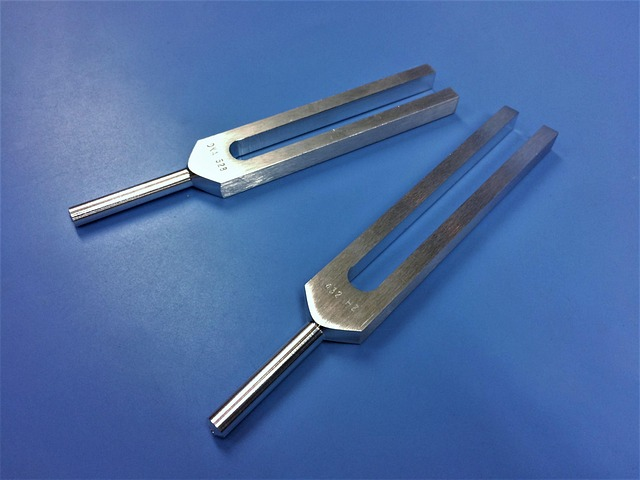
\includegraphics{tuning-fork}
  \caption[Tuning fork]{Tuning fork}
\end{marginfigure}
\subsection{Materials required}
\begin{enumerate}
\item Tuning fork
\item Rubber hammer
\item Bowl of water
\end{enumerate}
\subsection{Procedure}
Hold the tuning fork by its stem. Strike one prong of the tuning fork gently with a rubber hammer. Bring the vibrating tuning fork close to your ear.
\newthought{Observe:} Can you hear a sound? Touch the vibrating prongs gently with your finger. What do you feel when you touch the prongs? Touch the vibrating prongs lightly to the surface of the water. Observe the surface of the water. Do you see ripples on the surface of the water?
\begin{marginfigure}
  \centering
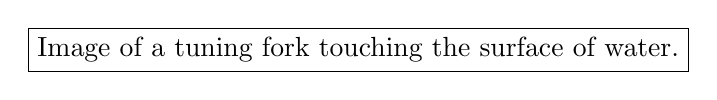
\begin{tikzpicture}
    \node[draw] at (0,0) {Image of a tuning fork touching the surface of water.};
  \end{tikzpicture}
  \caption{Ripples are formed on the surface of water when a vibrating tuning fork touches it.}
  \label{tuning-fork-water}
\end{marginfigure}

\marginnote{Did you know? Many quartz clocks and watches keep time using a small quartz crystal. This crystal is shaped like a tiny tuning fork.}